\documentclass{standalone}
\usepackage{tikz}
\usetikzlibrary{arrows.meta, decorations.pathreplacing}

\begin{document}

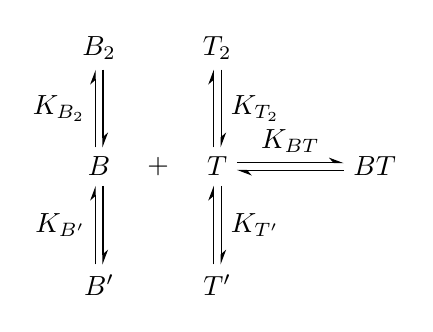
\begin{tikzpicture}[auto, node distance=2cm, >=Stealth]

    % Nodes
    \node (B2) {$B_2$};
    \node (B) [below of=B2, node distance=1.5cm] {$B$};
    \node (B') [below of=B, node distance=1.5cm] {$B'$};
    \node (T2) [right of=B2, node distance=1.5cm] {$T_2$};
    \node (T) [below of=T2, node distance=1.5cm] {$T$};
    \node (P) [left of=T, node distance=0.75 cm] {$+$};
    \node (T') [below of=T, node distance=1.5cm] {$T'$};

    \node (BT) [right of=T, node distance=2.0cm] {$BT$};
    
    % Harpoon Arrows with transform canvas
    \draw[<-, arrows={-Stealth[harpoon]}, transform canvas={xshift=-0.5mm}] (B) -- (B2) node[midway, left] {$K_{B_2}$};
    \draw[->, arrows={-Stealth[harpoon]}, transform canvas={xshift=0.5mm}] (B2) -- (B);
    
    \draw[<-, arrows={-Stealth[harpoon]}, transform canvas={xshift=-0.5mm}] (B') -- (B) node[midway, left] {$K_{B'}$};
    \draw[->, arrows={-Stealth[harpoon]}, transform canvas={xshift=0.5mm}] (B) -- (B');
    
    \draw[<-, arrows={-Stealth[harpoon]}, transform canvas={xshift=-0.5mm}] (T) -- (T2);
    \draw[->, arrows={-Stealth[harpoon]}, transform canvas={xshift=0.5mm}] (T2) -- (T) node[midway, right] {$K_{T_2}$};
    
    \draw[<-, arrows={-Stealth[harpoon]}, transform canvas={xshift=-0.5mm}] (T') -- (T);
    \draw[->, arrows={-Stealth[harpoon]}, transform canvas={xshift=0.5mm}] (T) -- (T') node[midway, right] {$K_{T'}$};

    % \hspace{0.5cm}
    
    \draw[<-, arrows={-Stealth[harpoon]}, transform canvas={yshift=0.5mm}] (T) -- (BT) node[midway, above] {$K_{BT}$};
    \draw[->, arrows={-Stealth[harpoon]}, transform canvas={yshift=-0.5mm}] (BT) -- (T);

\end{tikzpicture}

\end{document}
